% !TEX program = xelatex

\documentclass[xcolor=dvipsnames, xetex,serif]{beamer}
%\documentclass[handout,xetex,serif]{beamer} %ใช้บรรทัดนี้สำหรับปริ้นเอกสาร
\usepackage{color,amsmath,graphics,graphicx}
\usepackage{epsfig,amsfonts,graphics}
\usepackage{mathrsfs,hyperref}
\usepackage{subcaption,float,framed,algorithm2e,hyperref}
%===============================================
\usepackage{fontspec,xltxtra,xunicode}
\defaultfontfeatures{Scale=1.23}
\XeTeXlinebreaklocale “th_TH” % สำหรับตัดคำ
\setmainfont[Scale=1.23]{THSarabunNew}
% 1.23 เท่าคือจาก 12 pt บน LaTeX ให้เท่ากับ 16pt บน Word
%=====================================================
%\usepackage{pgfpages} %ใช้บรรทัดนี้สำหรับปริ้นเอกสาร
%\pgfpagesuselayout{4 on 1}[a4paper,border shrink=5mm,landscape]
%\pgfpagesuselayout{2 on 1}[a4paper,border shrink=5mm]
 %ใช้บรรทัดนี้สำหรับปริ้นเอกสาร

%%%%%%%%%%%%%%% THEOREM Environments %%%%%%%%%% 					
\newtheorem{conjecture}[theorem]{บทคาดการณ์}								
\newtheorem{remark}[theorem]{หมายเหตุ}										
\numberwithin{equation}{section}							
\renewcommand\tablename{ตารางที่}
\renewcommand\figurename{รูปที่}						
\renewcommand{\bibname}{บรรณานุกรม}						
\renewcommand{\indexname}{ดรรชนี}
\setbeamertemplate{caption}[numbered]	
\setbeamertemplate{theorems}[numbered]				
%%%%%%%%%%%%%%%%%%%%%%%%%%%%%%%%%%%%%%%%%%%%%%%

\mode<presentation>{
	\usetheme{Madrid}
	\usecolortheme[named=PineGreen]{structure}}
 \title[วิธีเชิงตัวเลขสำหรับต่อเติมภาพ]{\normalsize{ขั้นตอนวิธีเชิงตัวเลขชนิดใหม่สำหรับการต่อเติมภาพที่ใช้การแปรผันรวมกับการประยุกต์สำหรับซ่อมแซมภาพจิตรกรรมไทยโบราณและการลบบทบรรยายจากอนิเมะ\\A new numerical algorithm for TV-based image inpainting with its applications for restoring ancient Thai painting images and removing subtitles from animes}}
 \author[ภัคพล]{ภัคพล พงษ์ทวี}
 \institute[SU]{
 	ภาควิชาคณิตศาสตร์\\
 	มหาวิทยาลัยศิลปากร \\}
 \date[Project Progression]{การนำเสนอความก้าวหน้าโครงงานวิจัย ครั้งที่ 2\\
 	9 เมษายน 2562}
 
 \AtBeginSubsection[]{
 	\begin{frame}<beamer>
 		\frametitle{Outlines}
 		\tableofcontents [currentsection,currentsubsection]
	 \end{frame}
}
\begin{document}
	\begin{frame}
 		\titlepage 
	\end{frame}	 
	\begin{frame}
		\frametitle{ตัวแบบการต่อเติมภาพที่ใช้การแปรผันรวม}
		\begin{align*}
		\min_{u} \{ \mathcal{J}(u) = \frac{1}{2} \int_{\Omega}\lambda (u-z)^2 d\Omega +  \int_{\Omega}  |\nabla u|  d\Omega \}
		\end{align*}
		 \vspace{1cm}
		\begin{align*}
		\lambda=\lambda(\mathbf{x}) = \left \{ \begin{array}{ll}  \lambda_0, & x \in \Omega \textbackslash D \\ 0, & x \in D  \end{array} \right . 
		\end{align*}
		\let\thefootnote\relax\footnotetext{\tiny{T.F. Chan and J. Shen , “Mathematical models of local non-texture inpaintings”, SIAM Journal on Applied Mathematics, vol. 62, no. 3, pp. 1019–1043, 2001.}}	
	\end{frame} 
	\begin{frame}
		\frametitle{ตัวแบบการต่อเติมภาพเฉดสีเทาที่ใช้การแปรผันรวม (ต่อ)}
		\begin{align*}
		\min_{u} \{ \mathcal{J}(u) = \frac{1}{2} \int_{\Omega}\lambda (u-z)^2 d\Omega +  \int_{\Omega}  |\nabla u|  d\Omega \}
		\end{align*}
		$$ \Big \downarrow$$
		\begin{align*}
		\left \{ \begin{array}{ll}  - \nabla \cdot  \Big( \dfrac{\nabla u}{|\nabla u|} \Big) + \lambda (u-z) = 0,  & \hspace{1cm} \mathbf{x} \in (1,n)^2 \\ \dfrac{\partial u}{\partial \boldsymbol{n}} = 0, & \hspace{1cm} x \in \partial \Omega \end{array} \right .
		\end{align*}			
	\end{frame} 
	\begin{frame}
		\frametitle{ขั้นตอนวิธีเชิงตัวเลข}
		\begin{align*}
			u(\mathbf{x},t_{k+1})=u(\mathbf{x},t_{k})+\tau\left(\nabla \cdot\left(\dfrac{\nabla u (\mathbf{x},t_k)}{| \nabla u (\mathbf{x},t_k) | }\right) + \lambda(\mathbf{x})(u (\mathbf{x},t_k)-z(\mathbf{x})) \right)
		\end{align*}
		\begin{center}
		\textcolor{PineGreen}{วิธีที่ 1:} การเดินเวลา (Explicit time marching)
		\end{center}
		\begin{align*}
			- \nabla\cdot\left(\dfrac{\nabla u^{[\nu+1]}}{{| \nabla u |}^{[v]} }\right) + \lambda(u^{[\nu+1]}-z)  = 0,\ u^{[0]}=z
		\end{align*}
		\begin{center}
			\textcolor{PineGreen}{วิธีที่ 2:} ทำซ้ำจุดตรึง (Fixed point iteration)
		\end{center}
		\begin{align*}
			\min_{u,\boldsymbol{w}} \{ \mathcal{J}(u,\boldsymbol{w}) = \dfrac{1}{2} \int_{\Omega} \lambda(u-z)^2 d\Omega +  \int_{\Omega}  |\boldsymbol{w}|  d\Omega + \frac{\theta}{2} \int_{\Omega} (\boldsymbol{w} - \nabla u + \boldsymbol{b}) d\Omega \}
		\end{align*}
		\begin{center}
			\textcolor{PineGreen}{วิธีที่ 3:} สปริทเบรกแมน (Split Bregman)
		\end{center}
	\end{frame} 
	\begin{frame}
		\frametitle{ปัญหาเชิงตัวเลข}
			\begin{figure}[H]
			\centering
			
\includegraphics[width=0.2\linewidth]{images/grad_problem.png}
			\caption{ตัวอย่างภาพที่เกิดปัญหาเชิงตัวเลข}
			\label{image:rgb-space}
			\end{figure}
			\begin{align*}
			\tfrac{1}{| \nabla u |}=\tfrac{1}{\sqrt{u_x^2+u_y^2}} \rightarrow \infty
			\end{align*}
			\begin{align*}
			|\nabla u| \approx| \nabla u |_\beta=\sqrt{u_x^2+u_y^2+\beta},\ 0< \beta \ll 1
			\end{align*}
	\end{frame}
	\begin{frame}
		\frametitle{วิธีการสปริทเบรกแมน}
			\begin{align*}
		\min_{u,\boldsymbol{w}} \{ \mathcal{J}(u,\boldsymbol{w}) = \dfrac{1}{2} \int_{\Omega} \lambda(u-z)^2 d\Omega +  \int_{\Omega}  |\boldsymbol{w}|  d\Omega + \frac{\theta}{2} \int_{\Omega} (\boldsymbol{w} - \nabla u + \boldsymbol{b}) d\Omega \}
		\end{align*}
		$$ \Big \downarrow$$
		\begin{align*}
		u^{\text{New}}=\underset{u}{\arg\min} \{ \mathcal{J}_1(u) = \dfrac{1}{2} \int_{\Omega} \lambda(u-z)^2 d\Omega + \frac{\theta}{2} \int_{\Omega} (\boldsymbol{w}^{\text{old}} - \nabla u + \boldsymbol{b}^{\text{old}}) d\Omega \}
		\end{align*}
		\begin{align*}
		\boldsymbol{w}^{\text{New}}=\underset{\boldsymbol{w}}{\arg\min} \{ \mathcal{J}_2(\boldsymbol{w}) = \int_{\Omega}  | \boldsymbol{w}|  d\Omega  + \frac{\theta}{2} \int_{\Omega} (\boldsymbol{w} - \nabla u^{\text{New}} + \boldsymbol{b}^{\text{old}}) d\Omega \}
		\end{align*}
		\begin{align*}
		\boldsymbol{b}^{\text{New}}=\boldsymbol{b}^{\text{old}}+\nabla u^{\text{New}}-\boldsymbol{w}^{\text{New}}
		\end{align*}
	\end{frame}  
	\begin{frame}
		\frametitle{การวัดประสิทธิภาพ}
		\begin{align*}
			\text{PSNR}  = 10 \cdot log_{10} ( \frac{1}{\sqrt{\text{MSE}}} )  \hspace{1cm}
		\end{align*}
		\begin{center}
			Peak Signal Noise Ratio \textcolor{PineGreen}{(PSNR)} 
		\end{center}
		\vspace{1cm}
		\begin{align*}
			\text{SSIM}(u,\tilde{u}) = \frac{(2\mu_u\mu_{\tilde{u}} + 0.0001)(2\sigma_{u\tilde{u}} + 0.0009)}{(\mu_u^2+\mu_{\tilde{u}}^2+0.0001)(\sigma_u^2+\sigma_{\tilde{u}}^2+0.0009)}
		\end{align*}
		\begin{center}
			Structural Similarity \textcolor{PineGreen}{(SSIM)}
		\end{center}
	\end{frame}
	\begin{frame}
        \frametitle{ภาพสังเคราะห์}
        \begin{figure}[H]
            \centering
            \begin{subfigure}{0.15\linewidth}
                \centering
                
\includegraphics[width=0.9\linewidth]{images/image_inpaint_synthetic/case01-original.png}
            \end{subfigure}
            \begin{subfigure}{0.15\linewidth}
                \centering
                
\includegraphics[width=0.9\linewidth]{images/image_inpaint_synthetic/case02-original.png}
            \end{subfigure}
            \begin{subfigure}{0.15\linewidth}
                \centering
                
\includegraphics[width=0.9\linewidth]{images/image_inpaint_synthetic/case03-original.png}	
            \end{subfigure}
            \begin{subfigure}{0.15\linewidth}
                \centering
                
\includegraphics[width=0.9\linewidth]{images/image_inpaint_synthetic/case04-original.png}
            \end{subfigure}
            \begin{subfigure}{0.15\linewidth}
                \centering
                
\includegraphics[width=0.9\linewidth]{images/image_inpaint_synthetic/case05-original.png}	
            \end{subfigure}
            \caption{ภาพต้นฉบับ}
        \end{figure}
        \begin{figure}[H]
            \centering
            \begin{subfigure}{0.15\linewidth}
                \centering
                
\includegraphics[width=0.9\linewidth]{images/image_inpaint_synthetic/case01-toinpaint.png}
            \end{subfigure}
            \begin{subfigure}{0.15\linewidth}
                \centering
                
\includegraphics[width=0.9\linewidth]{images/image_inpaint_synthetic/case02-toinpaint.png}
            \end{subfigure}
            \begin{subfigure}{0.15\linewidth}
                \centering
                
\includegraphics[width=0.9\linewidth]{images/image_inpaint_synthetic/case03-toinpaint.png}
            \end{subfigure}
            \begin{subfigure}{0.15\linewidth}
                \centering
                
\includegraphics[width=0.9\linewidth]{images/image_inpaint_synthetic/case04-toinpaint.png}
            \end{subfigure}
            \begin{subfigure}{0.15\linewidth}
                \centering
                
\includegraphics[width=0.9\linewidth]{images/image_inpaint_synthetic/case05-toinpaint.png}
            \end{subfigure}
            \caption{ภาพที่จะทำการซ่อมแซม}
        \end{figure}
        \begin{align*}
            \text{รอบการทำซ้ำ} \leq 10,000 \text{รอบ} \hspace{1cm}
            \frac{|| u_{new} - u_{old} ||}{|| u_{new} ||} \geq 10^{-4}
        \end{align*}
    \end{frame}
    \begin{frame}
        \frametitle{ผลการต่อเติมภาพ}
        \begin{figure}[H]
            \centering
            \begin{subfigure}{0.15\linewidth}
                \centering
                
\includegraphics[width=0.9\linewidth]{images/result_ex1/timemarch01.png}
            \end{subfigure}
            \begin{subfigure}{0.15\linewidth}
                \centering
                
\includegraphics[width=0.9\linewidth]{images/result_ex1/timemarch02.png}
            \end{subfigure}
            \begin{subfigure}{0.15\linewidth}
                \centering
                
\includegraphics[width=0.9\linewidth]{images/result_ex1/timemarch03.png}
            \end{subfigure}
            \begin{subfigure}{0.15\linewidth}
                \centering
                
\includegraphics[width=0.9\linewidth]{images/result_ex1/timemarch04.png}
            \end{subfigure}
            \begin{subfigure}{0.15\linewidth}
                \centering
                
\includegraphics[width=0.9\linewidth]{images/result_ex1/timemarch05.png}
            \end{subfigure}
            \caption{ผลการซ่อมแซมจากวิธีการเดินเวลา}
        \end{figure}
        \begin{figure}[H]
            \centering
            \begin{subfigure}{0.15\linewidth}
                \centering
                
\includegraphics[width=0.9\linewidth]{images/result_ex1/fixpoint01.png}
            \end{subfigure}
            \begin{subfigure}{0.15\linewidth}
                \centering
                
\includegraphics[width=0.9\linewidth]{images/result_ex1/fixpoint02.png}
            \end{subfigure}
            \begin{subfigure}{0.15\linewidth}
                \centering
                
\includegraphics[width=0.9\linewidth]{images/result_ex1/fixpoint03.png}
            \end{subfigure}
            \begin{subfigure}{0.15\linewidth}
                \centering
                
\includegraphics[width=0.9\linewidth]{images/result_ex1/fixpoint04.png}
            \end{subfigure}
            \begin{subfigure}{0.15\linewidth}
                \centering
                
\includegraphics[width=0.9\linewidth]{images/result_ex1/fixpoint05.png}
            \end{subfigure}
            \caption{ผลการซ่อมแซมจากวิธีการทำซ้ำแบบจุดตรึง}
        \end{figure}
        \begin{figure}[H]
            \centering
            \begin{subfigure}{0.15\linewidth}
                \centering
                
\includegraphics[width=0.9\linewidth]{images/result_ex1/splitbergman01.png}
            \end{subfigure}
            \begin{subfigure}{0.15\linewidth}
                \centering
                
\includegraphics[width=0.9\linewidth]{images/result_ex1/splitbergman02.png}
            \end{subfigure}
            \begin{subfigure}{0.15\linewidth}
                \centering
                
\includegraphics[width=0.9\linewidth]{images/result_ex1/splitbergman03.png}
            \end{subfigure}
            \begin{subfigure}{0.15\linewidth}
                \centering
                
\includegraphics[width=0.9\linewidth]{images/result_ex1/splitbergman04.png}
            \end{subfigure}
            \begin{subfigure}{0.15\linewidth}
                \centering
                
\includegraphics[width=0.9\linewidth]{images/result_ex1/splitbergman05.png}
            \end{subfigure}
            \caption{ผลการซ่อมแซมจากวิธีการสปริทเบรกแมน}
        \end{figure}
    \end{frame}
	\begin{frame}
		\frametitle{ประสิทธิภาพของวิธีการเชิงตัวเลขทั้ง 3 วิธี}
		\begin{table}[H]
		\centering
		\captionsetup{justification=centering}
			\begin{tabular}[ht]{|l|c|c|c|c|}
				\hline
				วิธีการ  & เวลาประมวล  (วินาที) & PSNR (dB) & SSIM \\
				\hline
				การเดินเวลา & 120.68 & 16.72 & 0.9960 \\
				การทำซ้ำจุดตรึง & 74.81 & 38.67 & 0.9999 \\
				การสปริทเบรกแมน & 14.06 & 39.42 & 0.9999  \\
				\hline
			\end{tabular}
		\caption{แสดงการซ่อมแซมเฉลี่ยของวิธีการเชิงตัวเลข \\ โดยที่ $\lambda = 250, \beta = 10^{-5}, \tau = 10^{-5}, \theta = 5 $}
		\end{table}	
	\end{frame}
	\begin{frame}
		\frametitle{ขั้นตอนวิธีที่พัฒนาขึ้น}
		\begin{figure}[H]
			\centering
			\begin{subfigure}{0.4\linewidth}
				\centering
				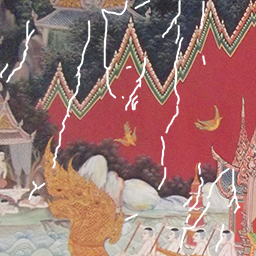
\includegraphics[width=0.8\linewidth]{images/our_method/preview_thaiart.png}
				\caption*{{\large การซ่อมแซมภาพศิลปะไทย}}
			\end{subfigure}
			\begin{subfigure}{0.4\linewidth}
				\centering
				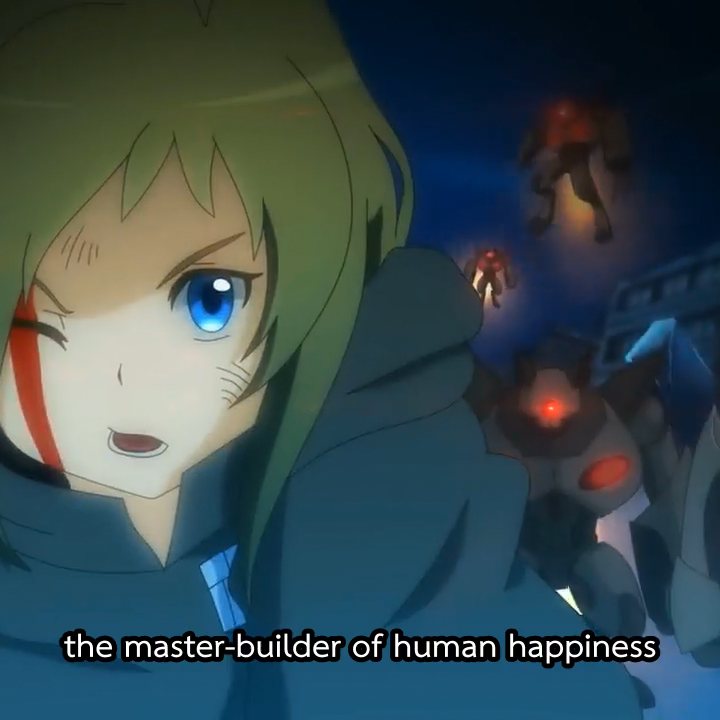
\includegraphics[width=0.8\linewidth]{images/our_method/preview_anime_square.png}
				\caption*{{\large การลบคำบรรยายอนิเมะ}}
			\end{subfigure}
		\end{figure}
	\end{frame}
	\begin{frame}
		\frametitle{คำตอบเริ่มต้น}
		\begin{figure}[H]
			\centering
			\begin{subfigure}{0.8\linewidth}
				\centering
				
\includegraphics[width=1\linewidth]{images/image_inital_solution.png}
			\end{subfigure}
			\caption{การใช้คำตอบเริ่มเต้นในวิธีการพีระมิดรูปภาพ}
		\end{figure}
	\end{frame}
	\begin{frame}
		\frametitle{ขั้นตอนวิธีสำหรับการซ่อมแซมภาพศิลปะไทย}
		\begin{figure}[H]
			\centering
			\begin{subfigure}{0.4\linewidth}
				\centering
				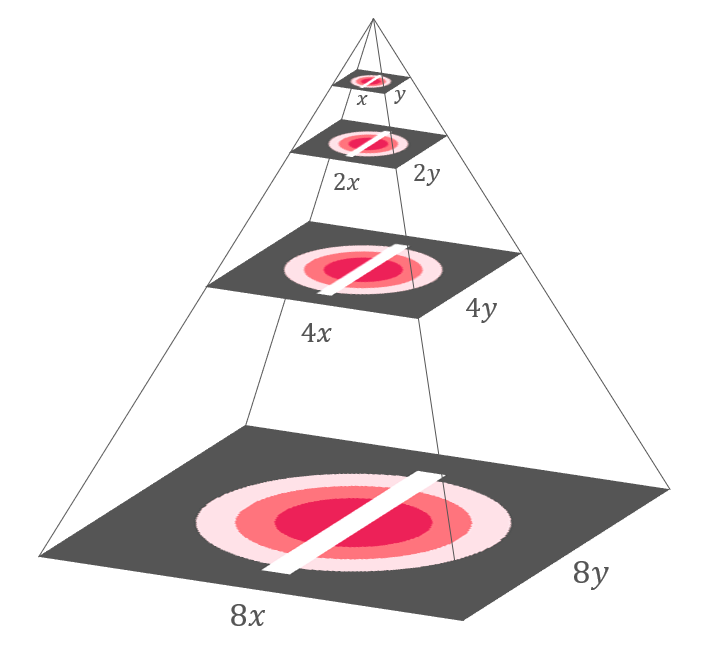
\includegraphics[width=0.8\linewidth]{images/method_thaiart/image_pyramid.png}
				\caption*{{\large พีระมิดรูปภาพ}}
			\end{subfigure}
			\begin{subfigure}{0.4\linewidth}
				\centering
				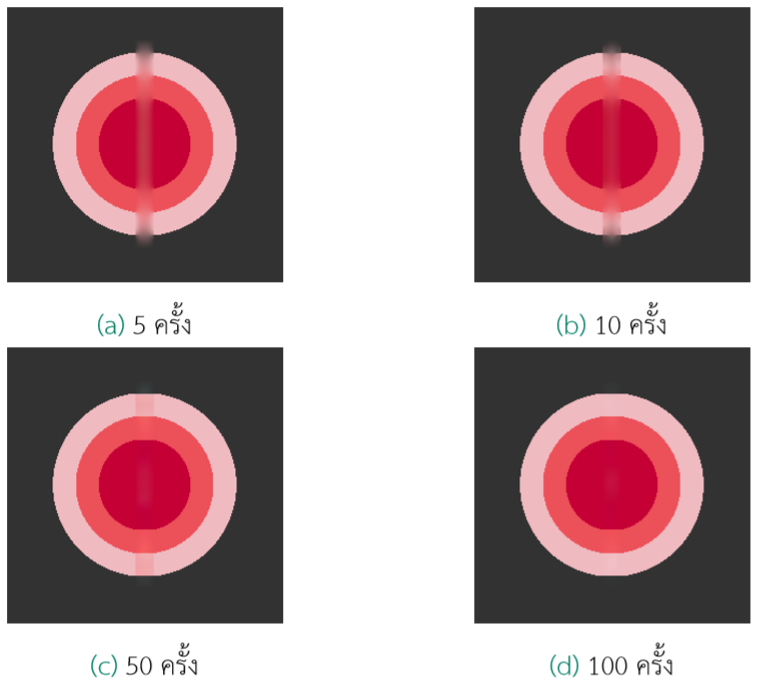
\includegraphics[width=0.8\linewidth]{images/method_thaiart/just10enough.png}
				\caption*{{\large จำกัดรอบทำซ้ำที่ชั้น}}
			\end{subfigure}
		\end{figure}	
	\end{frame}
	\begin{frame}
		\frametitle{ขั้นตอนวิธีสำหรับการซ่อมแซมภาพศิลปะไทย (ต่อ)}
		\begin{figure}[H]
			\centering
			\begin{subfigure}{0.5\linewidth}
				\centering
				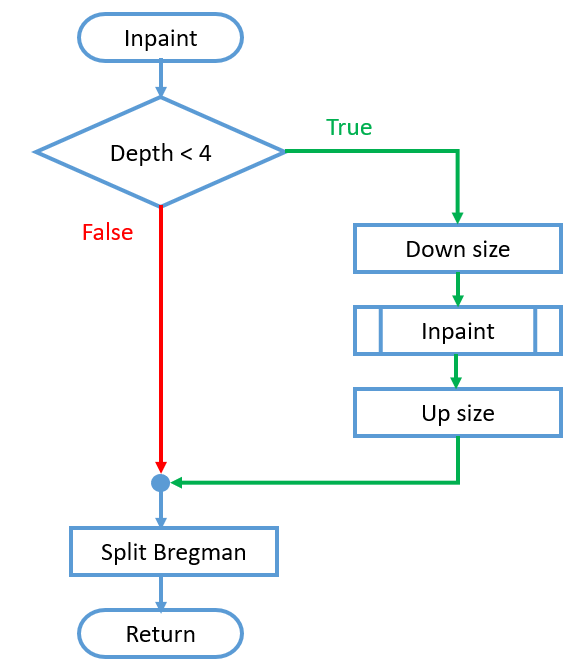
\includegraphics[width=1\linewidth]{images/method_thaiart/flowchart_thaiart.png}
			\end{subfigure}
			\caption{ผังงานขั้นตอนวิธีที่คิดค้นขึ้น}
		\end{figure}
	\end{frame}
	\begin{frame}
        \frametitle{การซ่อมแซมภาพจิตรกรรมไทยโบราณ}
        \begin{figure}[H]
            \centering
            \begin{subfigure}{0.15\linewidth}
                \centering
                
\includegraphics[width=0.9\linewidth]{images/thaiart/case01-original.png}
            \end{subfigure}
            \begin{subfigure}{0.15\linewidth}
                \centering
                
\includegraphics[width=0.9\linewidth]{images/thaiart/case02-original.png}
            \end{subfigure}
            \begin{subfigure}{0.15\linewidth}
                \centering
                
\includegraphics[width=0.9\linewidth]{images/thaiart/case03-original.png}
            \end{subfigure}		
            \begin{subfigure}{0.15\linewidth}
                \centering
                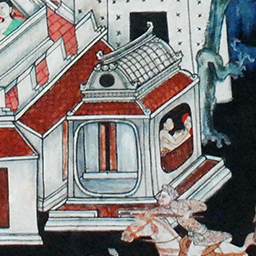
\includegraphics[width=0.9\linewidth]{images/thaiart/case04-original.png}
            \end{subfigure}
            \begin{subfigure}{0.15\linewidth}
                \centering
                
\includegraphics[width=0.9\linewidth]{images/thaiart/case05-original.png}
            \end{subfigure}
            \caption{ภาพต้นฉบับสำหรับใช้ในการทดสอบ}
        \end{figure}
        \begin{figure}[H]
            \centering
            \begin{subfigure}{0.15\linewidth}
                \centering
                
\includegraphics[width=0.9\linewidth]{images/thaiart/case01-toinpaint.png}
            \end{subfigure}
            \begin{subfigure}{0.15\linewidth}
                \centering
                
\includegraphics[width=0.9\linewidth]{images/thaiart/case02-toinpaint.png}
            \end{subfigure}
            \begin{subfigure}{0.15\linewidth}
                \centering
                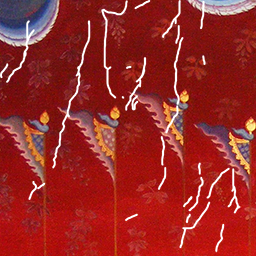
\includegraphics[width=0.9\linewidth]{images/thaiart/case03-toinpaint.png}			
            \end{subfigure}
            \begin{subfigure}{0.15\linewidth}
                \centering
                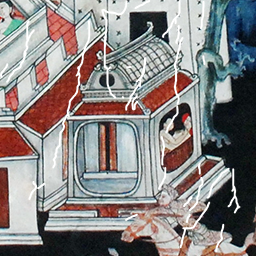
\includegraphics[width=0.9\linewidth]{images/thaiart/case04-toinpaint.png}			
            \end{subfigure}
            \begin{subfigure}{0.15\linewidth}
                \centering
                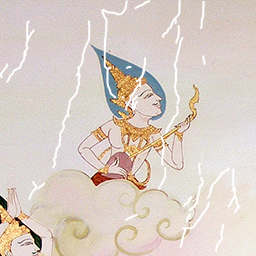
\includegraphics[width=0.9\linewidth]{images/thaiart/case05-toinpaint.png}			
            \end{subfigure}
            \caption{ภาพที่ทำให้เสียหาย}
        \end{figure}
    \end{frame}
    \begin{frame}
        \frametitle{ผลการซ่อมแซมภาพศิลปะไทย}
        \begin{figure}[H]
            \centering
            \begin{subfigure}{0.15\linewidth}
                \centering
                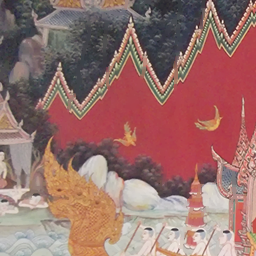
\includegraphics[width=0.9\linewidth]{images/result_ex4/splitbergman_case01.png}
            \end{subfigure}
            \begin{subfigure}{0.15\linewidth}
                \centering
                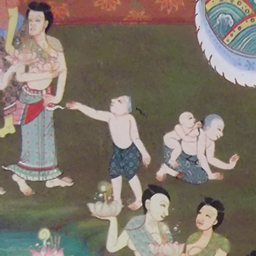
\includegraphics[width=0.9\linewidth]{images/result_ex4/splitbergman_case02.png}
            \end{subfigure}
            \begin{subfigure}{0.15\linewidth}
                \centering
                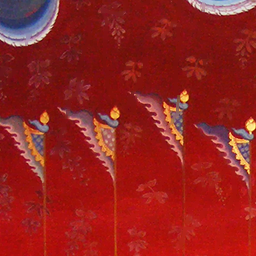
\includegraphics[width=0.9\linewidth]{images/result_ex4/splitbergman_case03.png}			
            \end{subfigure}
            \begin{subfigure}{0.15\linewidth}
                \centering
                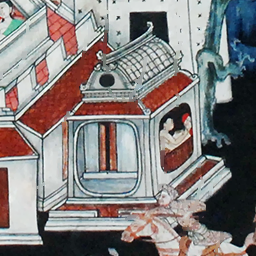
\includegraphics[width=0.9\linewidth]{images/result_ex4/splitbergman_case04.png}			
            \end{subfigure}
            \begin{subfigure}{0.15\linewidth}
                \centering
                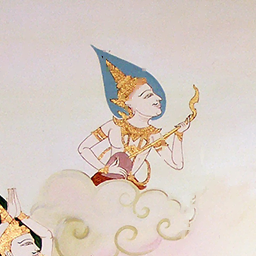
\includegraphics[width=0.9\linewidth]{images/result_ex4/splitbergman_case05.png}			
            \end{subfigure}
            \caption{ผลการซ่อมแซมโดยวิธีการสปริทเบรกแมน}
        \end{figure}
        \begin{figure}[H]
            \centering
            \begin{subfigure}{0.15\linewidth}
                \centering
                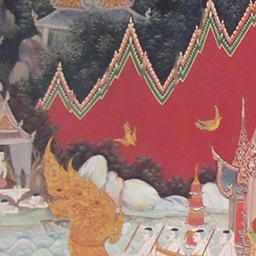
\includegraphics[width=0.9\linewidth]{images/result_ex4/multisplitbergman_case01.png}
            \end{subfigure}
            \begin{subfigure}{0.15\linewidth}
                \centering
                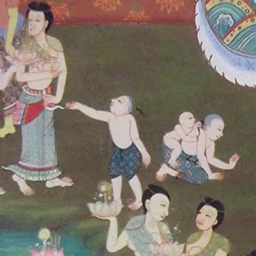
\includegraphics[width=0.9\linewidth]{images/result_ex4/multisplitbergman_case02.png}
            \end{subfigure}
            \begin{subfigure}{0.15\linewidth}
                \centering
                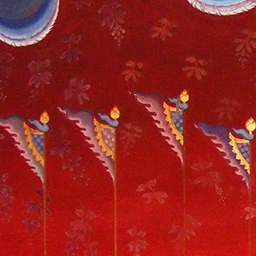
\includegraphics[width=0.9\linewidth]{images/result_ex4/multisplitbergman_case03.png}			
            \end{subfigure}
            \begin{subfigure}{0.15\linewidth}
                \centering
                \includegraphics[width=0.9\linewidth]{images/result_ex4/multisplitbergman_case04.png}			
            \end{subfigure}
            \begin{subfigure}{0.15\linewidth}
                \centering
                \includegraphics[width=0.9\linewidth]{images/result_ex4/multisplitbergman_case05.png}			
            \end{subfigure}
            \caption{ผลการซ่อมแซมโดยวิธีการที่พัฒนาขึ้น}
        \end{figure}
    \end{frame}
	\begin{frame}
		\frametitle{ผลการซ่อมแซมภาพศิลปะไทย}
		\begin{table}[H]
			\centering
			\begin{tabular}[ht]{|l|c|c|c|c|}
				\hline
				วิธีการ  & เวลาประมวล  (วินาที) & PSNR (dB) & SSIM \\
				\hline
				สปริทเบรกแมน & 2.72 & 34.89 & 1.0000 \\ 
				วิธีการที่พัฒนาขึ้น & 0.39 & 35.30 & 1.0000 \\
				\hline
			\end{tabular}
			\caption{แสดงผลการซ่อมแซมภาพศิลปะไทยในรูปค่าเฉลี่ย}
			\label{result:table-thaiart-summary}
		\end{table}	
	\end{frame}
	\begin{frame}
		\frametitle{ขั้นตอนสำหรับการลบคำบรรยายในอนิเมะ}
		\begin{figure}[H]
			\centering
			\begin{subfigure}{0.8\linewidth}
				\centering
				\includegraphics[width=1\linewidth]{images/method_anime/frame_sequence.png}
			\end{subfigure}
			\caption{ผังงานขั้นตอนวิธีที่คิดค้นขึ้น}
		\end{figure}
	\end{frame}
	\begin{frame}
		\frametitle{ขั้นตอนสำหรับการลบคำบรรยายในอนิเมะ (ต่อ)}
		\begin{figure}[H]
			\centering
			\begin{subfigure}{0.6\linewidth}
				\centering
				\includegraphics[width=1\linewidth]{images/method_anime/flowchart-skipandborrow.png}
			\end{subfigure}
			\caption{ผังงานขั้นตอนวิธีที่คิดค้นขึ้น}
		\end{figure}
	\end{frame}
	\begin{frame}
        \frametitle{ผลการลบคำบรรยาย}
        \begin{figure}[H]
            \centering
            \begin{subfigure}{0.4\linewidth}
                \centering
                \includegraphics[width=0.80\linewidth]{images/subtitle-remove/beforesubtitleremove.png}
                \caption{ก่อนลบคำบรรยาย}
                \label{image:ssim_location_prev}
            \end{subfigure}
            \begin{subfigure}{0.4\linewidth}
                \centering
                \includegraphics[width=0.80\linewidth]{images/subtitle-remove/aftersubtitleremove.png}
                \caption{หลังลบคำบรรยาย}
                \label{image:ssim_location_curr}
            \end{subfigure}
            %\caption{ก่อนลบคำบรรยายและหลังลบคำบรรยาย}
        \end{figure}
    \end{frame}
	\begin{frame}
        \frametitle{ผลการลบคำบรรยาย (ต่อ)}
        \begin{table}[H]
            \centering
            \captionsetup{justification=centering}
            \begin{tabular}[ht]{|l|c|c|c|c|}
                \hline
                วิธีการ  & เวลาประมวล  (วินาที) & PSNR (dB) & SSIM \\
                \hline
                สปริทเบรกแมน & 5073.08 & 32.88 & 0.9654 \\
                วิธีการที่พัฒนาขึ้น & 75.76 & 29.33 & 0.9454 \\
                \hline
            \end{tabular}
            \caption{ผลการลบบทบรรยายออกจากอนิเมะเฉลี่ย\\โดยวิธีการสปริทเบรกแมนและวิธีการที่พัฒนาขึ้น}
        \end{table}	
	\end{frame}
	\begin{frame}
		\frametitle{วิธีการดำเนินงาน}
		\scalebox{0.7}{\begin{tabular}[ht]{|l|c|c|c|c|c|c|c|c|c|c|c|c|}
				\hline
				&\multicolumn{7}{c|}{พ.ศ. 2561} &\multicolumn{5}{c|}{พ.ศ. 2562}\\
				\cline{2-13}
				แผนการดำเนินงาน&มิ.ย.&ก.ค.&ส.ค.&ก.ย.&ต.ค.&พ.ย.&ธ.ค.&ม.ค.&ก.พ.&มี.ค.&\textcolor{red}{\textbf{เม.ย.}}&พ.ค.\\
				\hline
				ศึกษาตัวแบบและขั้นตอนวิธีการต่อเติมภาพ-&x&x& & & & & & & & & &\\
				ที่ใช้การแปรผันรวมในเชิงลึก & & & & & & & & & & & &\\
				\hline
				พัฒนาขั้นตอนวิธีสำหรับการต่อเติมภาพ-& & &x&x&x&x& & & & & &\\
				ที่ใช้การแปรผันรวมชนิดใหม่ & & & & & & & & & & & &\\
				\hline
				ทดสอบขั้นตอนวิธีการต่อเติมภาพ- & & & &x &x&x& & & & & &\\
				ที่พัฒนาขึ้นโดยโปรแกรมคอมพิวเตอร์& & & & & & & & & & & &\\
				บนภาพสังเคราะห์และภาพจริง & & & & & & & & & & & &\\
				\hline
				อภิปรายผลที่ได้จากการทดลองเชิงตัวเลข & & & & & &x&x&x& & & &\\
				\hline
				สรุปผลการดำเนินงานวิจัย & & & & & & & & &x&x&\textcolor{red}{\textbf{x}}&x\\
				และจัดทำรูปเล่มฉบับสมบูรณ์ & & & & & & & & & & & &\\
				\hline
		\end{tabular}}
	\end{frame}
	\begin{frame}
        \frametitle{ลองซ่อมแซมภาพศิลปะ}
        \centering
        \begin{figure}[H]
            \centering
            \includegraphics[width=0.8\linewidth]{images/colab_sample.png}
            \caption{ลองใช้งานได้ที่ https://bit.ly/demothai}
        \end{figure}
	\end{frame}
	\begin{frame}
		\frametitle{โปรแกรมลบคำบรรยาย}
		\begin{figure}
			\includegraphics[width=0.8\linewidth]{images/demo_anime/file.png}
			\caption{ชุดไฟล์สำหรับลบคำบรรยาย (bit.ly/demo-anime-inpaint)}
		\end{figure}
		\begin{figure}
			\includegraphics[width=0.8\linewidth]{images/demo_anime/notepad.png}
			\caption{โค้ดภายใน SubtitleRemove.avs}
		\end{figure}
	\end{frame}
	\begin{frame}
		\centering
		\Huge{ขอขอบคุณ}
	\end{frame}
\end{document}





